\documentclass[ignorenonframetext,notheorems,aspectratio=1610]{beamer}
\usetheme[compress]{Madrid}
\usecolortheme{iwr}
\usepackage{../mathsim}
\tikzset{velox/.style={color=black,draw,fill=red,thick,%
    shape=diamond,aspect=.4,
    inner sep=1.3pt,transform shape}}
\tikzset{veloy/.style={color=black,draw,fill=red,thick,%
    shape=diamond,aspect=2.5,
    inner sep=1.3pt,transform shape}}
\tikzset{veloxy/.style={color=black,draw,fill=red,thick,%
    shape=star,star points=4,star point ratio=2.2,
    inner sep=1.3pt,transform shape}}
\tikzset{pressure/.style={color=black,draw,fill=cyan,thick,%
    shape=circle,inner sep=2pt,transform shape}}
\tikzset{velo/.style={transform shape,double=red,arrows={-Stealth[open,fill=red]}}}

%% Macros for drawing degrees of freedom for different shapes/elements.
%% Arguments are always:
%%   #1: Starting point
%%   #2: End point
%%   #3: polynomial degree
%%   #4: node settings

\tikzset{pics/edgenormal/.style args={#1/#2/#3/#4}{%
    code={%
      \draw #1 -- #2
      node foreach \x [evaluate=\x as \xval] in {1,...,#3} [#4,sloped,pos=\xval/(#3+1)] {};
      }
}}


%% Macros for drawing degrees of freedom for different shapes/elements.
%% Arguments are always:
%%   #1: polynomial degree
%%   #2: node settings

\tikzset{pics/tripile/.style args={#1/#2}{%
    code={%
      \coordinate (top) at (0,#1);
      \foreach \i in{0,...,#1}
      \foreach \j in{0,...,\i}
      {
        \tikzmath{
          \y = .3*(2/3*#1-\i)*cos(30);
          \x = .3*(\i/2-\j);
        }
        \node[#2] at (\x,\y) {};
      }
    }
}}

\tikzset{pics/tensor/.style args={#1/#2/#3}{%
    code={%
      \coordinate (top) at (0,#1);
      \foreach \i in{0,...,#1}
      \foreach \j in{0,...,#2}
      {
        \tikzmath{
          \y = 2*(\i+1)/(#1+2);
          \x = 2*(\j+1)/(#2+2);
        }
        \node[#3] at (\x,\y) {};
      }
    }
}}

\tikzset{pics/pfem/.style args={#1/#2}{%
    code={%
      \tikzmath{ \ytop=2*cos(30); }
      \coordinate (top) at (0,\ytop);

      \foreach \i in{0,...,#1}
      \foreach \j in{0,...,\i}
      {
        \tikzmath{
          \y = \ytop-\ytop*\i/#1;
          \x = 2*(\i/2-\j)/#1+1;
        }
        \node[#2] at (\x,\y) {};
      }
    }
}}

\tikzset{pics/qfem/.style args={#1/#2}{%
    code={%
      \foreach \i in{0,...,#1}
      \foreach \j in{0,...,#1}
      {
        \tikzmath{
          \y = 2-2*\i/#1;
          \x = 2-2*\j/#1;
        }
        \node[#2] at (\x,\y) {};
      }
    }
}}

%%% Local Variables:
%%% mode: latex
%%% TeX-master: "all"
%%% End:

\mathtoolsset{showonlyrefs}
\excludecomment{solution}
\externaldocument{main}

\makeatletter
\def\BT@with[#1]#2(#3){\begin{block}{#3 \capitalizewords{#2} (#1)}}
\def\BT@without#1(#2){\begin{block}{#2 \capitalizewords{#1}}}
\def\endblocktheorem{\end{block}}
\makeatother
\def\mylabel#1{}
\let\label\mylabel
%\renewcommand{\label}[1]{}
\renewcommand{\eqref}[1]{(\ref{#1})}
\renewcommand{\define}[1]{\textbf{#1}}

\begin{document}
\frame{\tableofcontents}
\section{From elliptic to mixed problems}
\frame {\input {blocks/Notation-vector-diff-operators.tex}}
\frame {\input {blocks/Definition-strain-tensor.tex}}
\frame {\input {blocks/Definition-hooke.tex}}
\frame {\input {blocks/Definition-weak-lame-navier.tex}}
\frame {\input {blocks/Problem-frobenius.tex}}
\frame {\input {blocks/Assumption-korn-inequality.tex}
  \input {blocks/Lemma-korn.tex}}
\frame {\small\input {blocks/Problem-elasticity-standard.tex}}

\begin{frame}
  \frametitle{Example: hanging sheet}
  \centering
  \begin{tabular}{ccc}
    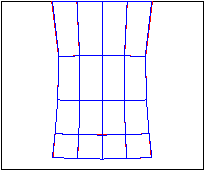
\includegraphics[width=.25\textwidth]{./graph/elasticity/stalactite-0}
    &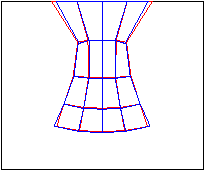
\includegraphics[width=.25\textwidth]{./graph/elasticity/stalactite-1}
    &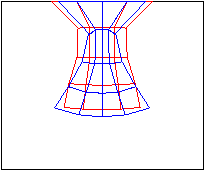
\includegraphics[width=.25\textwidth]{./graph/elasticity/stalactite-2}
    \\
    $\lambda = 1$&$\lambda = 10$&$\lambda = 100$
    \\\\
    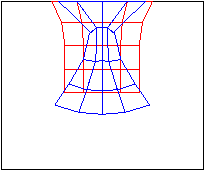
\includegraphics[width=.25\textwidth]{./graph/elasticity/stalactite-3}
    &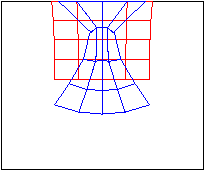
\includegraphics[width=.25\textwidth]{./graph/elasticity/stalactite-4}
    &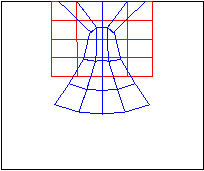
\includegraphics[width=.25\textwidth]{./graph/elasticity/stalactite-5}
    \\
    $\lambda = 1000$&$\lambda = 10000$&$\lambda = 100000$
  \end{tabular}
\end{frame}
\frame {\input {blocks/Definition-displacement-pressure.tex}}
\frame {\input {blocks/Definition-lame-navier-strong.tex}}
\frame {\input {blocks/Definition-saddle-point-operators.tex}}
\frame {\input {blocks/Definition-saddle-point-abstract.tex}}
\frame {\input {blocks/Notation-saddle-point-form.tex}}
\frame {\input {blocks/Definition-schur-complement.tex}
  \input {blocks/Lemma-schur-complement1.tex}}
\frame {\input {blocks/Lemma-schur-definiteness.tex}}
\frame {\input {blocks/Definition-stokes-eq1.tex}}
\frame {\input {blocks/Definition-solenoidal.tex}}
\frame {\input {blocks/Lemma-stokes-equivalence.tex}}
\frame {\input {blocks/Definition-stokes-eq2.tex}}
\frame {\input {blocks/Definition-stokes-boundary2.tex}}
\frame {\input {blocks/Lemma-divergence-compatibility.tex}
\input {blocks/Notation-pressure-constant.tex}}
\frame {\input {blocks/Theorem-minimization.tex}}
\frame {\input {blocks/Definition-reduced-problem.tex}
\input {blocks/Lemma-reduced-wellposedness.tex}}
\frame {\input {blocks/Theorem-lagrange-multiplier.tex}}
\frame {\input {blocks/Problem-lagrange-multiplier.tex}}
\frame {\input {blocks/Corollary-stokes-lagrange.tex}}

\section{Conditions for well-posedness}
\frame {\input {blocks/Problem-unbounded-inverse.tex}}
\frame {\input {blocks/Problem-lax-milgram-not-applicable.tex}}
\frame {\input {blocks/Theorem-la-invertible.tex}}
\frame {\input {blocks/Theorem-svd.tex}}
\frame {\input {blocks/Corollary-svd-order.tex}}
\frame {\input {blocks/Definition-ker-range-rn.tex}
\input {blocks/Definition-orthogonal1.tex}}
\frame {\input {blocks/Lemma-ker-coker-rn.tex}
\input {blocks/Corollary-ker-coker-iso.tex}
\input {blocks/Corollary-svd-infsup.tex}}
\frame {\input {blocks/Definition-infsup1.tex}
\input {blocks/Lemma-infsup2.tex}
\input {blocks/Problem-inf-sup-equivalence.tex}}
\frame {\input {blocks/Definition-polar-orthogonal.tex}
\input {blocks/Lemma-orthogonal-closed.tex}
\input {blocks/Theorem-orthogonal-complement.tex}}
\frame {\input {blocks/Definition-orthogonal-projection.tex}}
\frame {\input {blocks/Lemma-polar-orthogonal-hilbert.tex}}
\frame {\input {blocks/Theorem-closed-range.tex}}
\frame {\input {blocks/Theorem-open-mapping.tex}
\input {blocks/Lemma-closed-infsup.tex}}
\frame {\input {blocks/Theorem-infsup-well-equivalence.tex}}
\frame {\input {blocks/Corollary-infsup-well-posedness1.tex}}
\frame {\input {blocks/Theorem-infsup-well-posedness2.tex}}
\frame {\input {blocks/Theorem-infsup-mixed1.tex}}
\frame {\input {blocks/Theorem-infsup-mixed2.tex}}
\frame {\input {blocks/Problem-inhomogeneous-continuity.tex}}
\frame {\input {blocks/Assumption-mixed-elliptic.tex}}

\subsection{Galerkin approximation of mixed problems}

\frame {\input {blocks/Definition-kerbh.tex}}
\frame {\input {blocks/Definition-mixed-galerkin.tex}}
\frame {\input {blocks/Theorem-galerkin-mixed-u-kerbh.tex}}
\frame {\input {blocks/Corollary-galerkin-mixed-u-kerb.tex}}
\frame {\input {blocks/Theorem-galerkin-mixed-existence-p.tex}}
\frame {\input {blocks/Problem-infsup-uniform.tex}}
\frame {\input {blocks/Lemma-fortin.tex}}
\frame {\input {blocks/Assumption-mixed-elliptic-stabilized.tex}}
\frame {\input {blocks/Theorem-mixed-stabilized-well-posed.tex}}
\frame {\input {blocks/Definition-mixed-residual.tex}}
\frame {\input {blocks/Corollary-mixed-residual-bounded.tex}}
\frame {\input {blocks/Lemma-stabilized-mixed-approximation.tex}}
\frame {\input {blocks/Corollary-stabilized-mixed-convergence.tex}}

\section{Stokes equations}

\frame {\input {blocks/Lemma-stokes-a-elliptic.tex}}
\frame {\input {blocks/Lemma-stokes-helmholtz.tex}
  \input {blocks/Lemma-stokes-grad.tex}}
\frame {\input {blocks/Corollary-stokes-iso.tex}
  \input {blocks/Theorem-stokes-infsup.tex}}
\frame {\input {blocks/Theorem-stokes-convergence.tex}}
\frame {\input {blocks/Corollary-stokes-convergence2.tex}}
\frame {\input {blocks/Problem-checker-board.tex}}

\begin{frame}
  \frametitle{Example: one-dimensional $P_1-P_1$ elements}
  \begin{center}
      \includegraphics[width=.7\textwidth]{./fig/p1-p1-1d}
  \end{center}
\end{frame}

\begin{frame}
  \frametitle{Small patches with Dirichlet boundary}
  \begin{center}
    \hfill
    \includegraphics[width=.3\textwidth]{./fig/patch1.tikz}
    \hfill
    \includegraphics[width=.3\textwidth]{./fig/patch2.tikz}
    \hfill\mbox{}
  \end{center}
\end{frame}

\begin{frame}
  \frametitle{Checkerboard modes}
  
\end{frame}

\subsection{MINI element}
\frame {\input {blocks/Definition-barycentric-coordinates.tex}}

\begin{frame}
  \frametitle{The $P_1$ element in barycentric coordinates}
  \begin{columns}
    \begin{column}{.5\textwidth}
      \begin{center}
        \includegraphics[width=.6\textwidth]{./fig/p1-p.tikz}
      \end{center}
    \end{column}
    \begin{column}{.5\textwidth}
      \begin{gather*}
        \phi_i = \lambda_i,
        \quad i=0,1,2
      \end{gather*}
    \end{column}
  \end{columns}
\end{frame}

\begin{frame}
  \frametitle{The $P_2$ element in barycentric coordinates}
  \begin{columns}
    \begin{column}{.5\textwidth}
      \begin{center}
        \includegraphics[width=.6\textwidth]{./fig/p2-p.tikz}
      \end{center}
    \end{column}
    \begin{column}{.5\textwidth}
      \begin{xalignat*}2
        \phi_{ii} &= 2\lambda_i^2 - \lambda_i,
        &i&=0,1,2\\
        \phi_{ij} &= 4\lambda_i\lambda_j
        &j&\neq i
      \end{xalignat*}
    \end{column}
  \end{columns}
\end{frame}

\begin{frame}
  \frametitle{The $P_3$ element in barycentric coordinates}
  \begin{columns}
    \begin{column}{.5\textwidth}
      \begin{center}
        \includegraphics[width=.6\textwidth]{./fig/p3-p.tikz}
      \end{center}
    \end{column}
    \begin{column}{.5\textwidth}
      \begin{xalignat*}2
        \phi_{iii} &= \tfrac12 \lambda_i(3\lambda_i-1)(3\lambda_i-2)
        &i&=0,1,2\\
        \phi_{ij} &= \tfrac92\lambda_i\lambda_j(3\lambda_j-1)
        &j&\neq i\\
        \phi_0 &= 27\lambda_0\lambda_1\lambda_2
      \end{xalignat*}
    \end{column}
  \end{columns}
\end{frame}

\frame {\input {blocks/Notation-piecewise-polynomial-spaces.tex}}
\frame {\input {blocks/Definition-h1-bubble-space.tex}}
\frame {\input {blocks/Definition-mini-element-p.tex}}
\frame {\input {blocks/Lemma-fortin-construction-1.tex}}
\frame {\input {blocks/Assumption-h1-stable-interpolation.tex}}
\frame {\input {blocks/Definition-locally-quasi-uniform.tex}
  \input {blocks/Assumption-locally-quasi-uniform.tex}}
\frame {\input {blocks/Theorem-mini-stability.tex}}
\frame {\input {blocks/Notation-broken-bilinear-form.tex}}
\frame {\input {blocks/Lemma-mini-stabilized.tex}}
\frame {\input {blocks/Problem-quadrilateral-mini.tex}}
\frame {\input {blocks/Problem-mini-3d.tex}}
\frame {\input {blocks/Definition-higher-order-bubble.tex}}
\frame {\input {blocks/Theorem-higher-order-bubble.tex}
  \input {blocks/Corollary-pk-bubble.tex}}

\subsection{P2-P0}

\frame {\input {blocks/Definition-p2-p0-element.tex}
  \input {blocks/Lemma-p2-p0-stability.tex}}
\frame {\input {blocks/Theorem-p2-p0-convergence.tex}}
\frame {\input {blocks/Problem-q2-q0.tex}}
\frame {\input {blocks/Lemma-bubble-discontinuous.tex}}
\frame {\input {blocks/Corollary-bubble-p2.tex}
  \input {blocks/Corollary-pk-pk2.tex}}

\frame {\input {blocks/Theorem-discontinuous-pressure-normal-velocity.tex}}
\frame {\input {blocks/Corollary-qk-pk1.tex}}
\frame {\input {blocks/Definition-moment-dofs-qk-2d.tex}}
\frame {\input {blocks/Definition-moment-dofs-qk-3d.tex}}
\frame {\input {blocks/Example-qk-pk1.tex}}

\subsection{The Hood-Taylor elements}

\frame {\input {blocks/Definition-hood-taylor.tex}}
\frame {\input {blocks/Example-hood-taylor-triangle.tex}}
\frame {\input {blocks/Example-hood-taylor-quad.tex}}
\frame {\input {blocks/Definition-macro-equivalence.tex}}
\frame {\input {blocks/Problem-reference-macros.tex}}
\frame {\input {blocks/Definition-macro-spaces.tex}}
\frame {\input {blocks/Definition-verfuerth-norm.tex}}
\frame {\input {blocks/Definition-macro-seminorm.tex}}
\frame {\input {blocks/Lemma-macro1.tex}}
\frame {\input {blocks/Lemma-macro-local.tex}}
\frame {\input {blocks/Problem-macro-local.tex}}
\frame {\input {blocks/Lemma-verfuerth1.tex}}
\frame {\input {blocks/Lemma-verfuerth2.tex}}
\frame {\input {blocks/Theorem-hood-taylor-stability.tex}}

\frame {\input {blocks/Lemma-patch-test-triangle.tex}}
\frame {\input {blocks/Lemma-patch-test-quad.tex}}

\subsection{Almost incompressible elasticity}

\frame {\input {blocks/Lemma-reduced integration.tex}}
\frame {\input {blocks/Theorem-mixed-stabilized-well-posed.tex}}
\frame {\input {blocks/Corollary-stabilized-mixed-convergence.tex}}

\section{Mixed formulation of elliptic problems}
\frame {\input {blocks/Definition-primal-mixed.tex}}
\frame {\input {blocks/Definition-hdiv.tex}}
\frame {\input {blocks/Definition-dual-mixed.tex}}
\frame {\input {blocks/Theorem-Hdiv-separable.tex}
  \input {blocks/Theorem-Hdiv-trace.tex}}
\frame {\input {blocks/Problem-trace-dnu.tex}}
\frame {\input {blocks/Theorem-Hdiv-trace-surjective.tex}
  \input {blocks/Theorem-Hdiv-trace-kernel.tex}}
\frame {\input {blocks/Theorem-Hdiv-helmholtz.tex}}
\frame {\input {blocks/Problem-mixed-inhomogeneous-bc.tex}}
\frame {\input {blocks/Lemma-darcy-reduced-wellposed.tex}}
\frame {\input {blocks/Lemma-darcy-infsup.tex}
  \input {blocks/Theorem-darcy-well-posed.tex}}
\frame {\small\input {blocks/Theorem-infsup-mixed2.tex}}

\subsection{Discretization of dual mixed problems}

\frame {\input {blocks/Lemma-normal-continuity.tex}}
\frame {\input {blocks/Definition-rt-simplex.tex}}
\frame {\input {blocks/Example-rt-simplex.tex}}
\frame {\input {blocks/Lemma-rt-simplex-1.tex}}
\frame {\input {blocks/Lemma-rt-simplex-dimension.tex}}
\frame {\input {blocks/Lemma-rt-simplex-unisolvence.tex}}

\frame {\input {blocks/Definition-bdm-simplex.tex}}
\frame {\input {blocks/Example-bdm-simplex.tex}}
\frame {\input {blocks/Lemma-bdm-simplex-unisolvence.tex}}
\frame {\input {blocks/Definition-canonical-interpolation.tex}}
\frame {\input {blocks/Lemma-commuting-diagram-hdiv.tex}}

\subsection{Quarilaterals and hexahedra}

\frame {\input {blocks/Notation-recap-reference-transform.tex}}
\frame {\input {blocks/Definition-Piola-transform.tex}}
\frame {\input {blocks/Lemma-Piola-transform-integrals.tex}
  \input {blocks/Problem-Piola-transform-integrals.tex}}
\frame {\input {blocks/Notation-tensor-product-polynomials.tex}}
\frame {\input {blocks/Definition-rt-quad.tex}}
\frame {\input {blocks/Example-rt-quad.tex}}
\frame {\input {blocks/Lemma-rt-quad-1.tex}}
\frame {\input {blocks/Definition-bdm-quad.tex}}
\frame {\input {blocks/Example-bdm-quad.tex}}
\frame {\input {blocks/Lemma-bdm-quad.tex}
  \input {blocks/Problem-bdm-quad.tex}}
\frame {\input {blocks/Corollary-darcy-convergence-affine.tex}}

\section{Divergence conforming DG}

\end{document}

%%% Local Variables:
%%% mode: latex
%%% TeX-master: t
%%% End:
